\chapter{Chapter 5 Supplemental Information}
\label{sec:app5}
\raggedbottom

\clearpage

\section{Supplemental Methods}

\subsection{Satellite tagging and data} \label{sec:a5satdata}

Adult male blue sharks (mean 264 cm fork length, range 220-313 cm) were tagged near Montauk, New York during Summer 2013 and 2014 (n=2) and Cape Cod, MA during Fall 2015 and 2016 (n=17; Table \ref{tab:a5t1}). All were tagged with fin-mounted Smart Position or Temperature Transmitting (SPOT, Wildlife Computers) tags, and we deployed pop-up satellite archival transmitting (PSAT, model miniPAT, Wildlife Computers) tags, in addition to SPOT tags, on the individuals near Cape Cod (n=17; Table \ref{tab:a5t1}). Sharks were captured on rod and reel and brought onboard the fishing vessel where they were ventilated with a seawater hose and the hook was removed. SPOT tags were affixed to the dorsal fin using nylon bolts and contained a wet/dry switch that activated at the surface to transmit to the Argos satellite network from which a Doppler-based position was calculated. PSATs were tethered with a stainless steel wire to an intramuscular T-bar style spear tip (n=16) or a nylon umbrella dart (n=3). \textit{In situ} measurements of pressure, temperature and light levels were collected every 15 seconds throughout the PSAT deployments and aggregated for satellite transmission. Archived depth and temperature data were transmitted as 4 summarized products: (1) time-at-temperature and (2) time-at-depth histograms for 12 bins every 24 hours; (3) depth-temperature profiles at 16 representative depths every 24 hours; (4) depth time series at 2.5 minute resolution. PSATs were programmed to detach after 180 days and transmit these summarized data products, along with daily light level data for geolocation, via the Argos satellite system.

Resulting SPOT-tag locations were processed with a Kalman filtering algorithm by Collecte Localisation Satellites \citep{Lopez2014} and subsequently assigned error flags called location classes (LC): LC 3, <250 m; LC 2, 250-500 m; LC 1, 500-1500 m; LC 0, >1500 m for classes 3, 2, 1, 0. Additional classes A, B represent positions derived from less than 4 satellite messages which result in no estimates of spatial accuracy from CLS; however, recent work on several marine species and platforms suggests error for A, B classes is order 1-10 km and nearly always < 20 km \citep{Lopez2014}. Location class Z positions were considered invalid and removed from further analysis \citep{CLS2016}. Remaining positions were filtered using a speed filter (4 $m s^{-1}$) from the \texttt{trip} package \citep{Sumner2009} to remove unrealistic locations. The filtered Argos data were fit in a hierarchical fashion with a two-state switching state-space model (SSM) to estimate locations from the noisy Argos data, infer behavioral state and standardize the location time series (6 hr resolution) \citep{Jonsen2016}. The SSM combines a process model that estimates movement parameters and an observation model that accounts for spatial uncertainty using Markov Chain Monte Carlo (MCMC). The model inferred a behavior state based on fitted movement parameters (correlation, $\gamma$ and turn angle, $\theta$). Resident behavior (often referred to as area-restricted search or foraging) was characterized by $\theta$ near 180$^{\circ}$ and $\gamma$ near 0 (short steps with large turn angles), while traveling (or transit) behavior produces movements in which $\theta$ is near 0$^{\circ}$ and $\gamma$ near 1 (long, relatively straight tracks) between consecutive steps in the individual trajectories. Blue shark tracks were divided into trajectories for which data gaps were no longer than 4 days. Models were fit in JAGS \citep{Plummer2004} using the \texttt{bsam} package \citep{Jonsen2016} for \texttt{R} \citep{RDevelopmentCoreTeam2015}. The models were fit with a 6 hour time step using two MCMC chains of 60,000 samples from which the first 40,000 were discarded as burn-in. Posterior inference was performed from the remaining 20,000 samples per chain after thinning by a factor of 20 to reduce within-chain sample autocorrelations, yielding a final 2,000 samples from the joint posterior. Model convergence was assessed using criteria outlined in \citep{Jonsen2016} and included$\colon$ posterior samples were stationary, MCMC chains were well-mixed, within-chain autocorrelation was low and the Brooks-Gelman-Rubin potential scale reduction factors ($\hat{r}$) were $\leq$ 1.1.

\subsection{Oceanographic data}

To quantify associations between blue sharks and mesoscale eddies, we used the Mesoscale Eddy Trajectory Atlas distributed by Archiving Validation and Interpretation of Satellite and Oceanographic Data (AVISO; \href{https://www.aviso.altimetry.fr/en/data/products/value-added-products/global-mesoscale-eddy-trajectory-product.html}{https://www.aviso.altimetry.fr/en/data/products/value-added-products/global-mesoscale-eddy-trajectory-product.html)} that describes daily tracks of coherent mesoscale structures (CMS) based on maps of surface altimetry \citep{Chelton2011}. Eddies with lifetimes greater than 4 weeks (28 days) are tracked based on their signatures in sea-level anomaly (SLA) fields. Prior to the identification and tracking of mesoscale eddies, the SLA fields are high-pass filtered using a 20$^\circ$ x 10$^\circ$ (longitude x latitude) 2D weighted least-squares regression (LOESS) smoother to remove the effects of seasonal heating and cooling \citep{Chelton2011} as:

\begin{equation}
SSH = SLA - \left<SLA\right>
\label{eq:a5ssh}
\end{equation}

where the $<>$ operator indicates spatial smoothing. We developed a meander filter for the Gulf Stream region (see Section \ref{sec:a5eddycoll}) using daily, 0.25$^\circ$ resolution absolute dynamic topography (ADT) data from AVISO which is generated by satellite-derived anomalies from the mean dynamic topography surface \citep{Rio2011}. Daily, 1 km sea surface temperature (SST) data was acquired from NASA JPL's Multi-scale Ultra-high Resolution (MUR) product. SRTM30+ bathymetry from Scripps was downloaded from NOAA CoastWatch server (ERDDAP id: srtm30plus) \citep{Becker2009}.

\subsection{Eddy collocation} \label{sec:a5eddycoll}

Eddy occupation was quantified using a subset of the track data to include those positions that were in the Gulf Stream, a well-known region of mesoscale activity, in water deeper than 2000 m and that corresponded to the temporal limits of the eddy tracking dataset (Jan 1993 - Jan 2017). To focus our analysis on eddies, we developed a two-step meander filter for the Gulf Stream region \citep{Gaube2017DSR} in which we: 

\begin{enumerate} 
\item defined a mask 1$^\circ$ north and 2$^\circ$ south of the GS north wall (40 cm ADT contour). Those features in which the core of the CMS was within the meander mask were considered meanders and removed from the remainder of the analysis. 
\item calculated net zonal displacement of eddies and removed those that exhibited primarily eastward displacement, following \citep{Gaube2017DSR}, using a 3-day rolling window. 
\end{enumerate}

Shark locations were collocated to the nearest eddy identified in the eddy atlas (excluding meanders as described above) following \citep{Gaube2017}. We also used a maximum distance from the eddy center of 200 km or 2.5 times the length of the eddy radius to prevent collocation to eddies from an unreasonable distance to be biologically-relevant.

To assess differences in the distribution of blue sharks within anticyclonic and cyclonic eddies, we constructed histograms of blue shark location as a function of radial distance from the eddy center, resulting in number of shark positions per unit area of an annulus defined by the radial distance from the eddy center. To determine if individuals are more likely to be associated with the core, interior or periphery of eddies of either polarity, we defined eddy subregions by the normalized distance $r$ from the eddy SLA extremum, where the inner-core is defined as $r \leq L_s/2$, the outer core as $L_s/2 < r \leq L_s$ and the eddy interior includes both the inner and outer core $r \leq L_s$. The eddy periphery is defined as $L_s < r \leq 2L_s$ and the area outside of an eddy as $r > 2L_s$ \citep[see Fig. 2 in][]{Gaube2017}.

We compared observed movements to two null models of eddy use by collocating simulated tracks and drifter data to the eddy field as described above. We generated 100 correlated random walk (CRW) simulations per blue shark using the distributions of turn angles and step lengths from each individual's observed movement data \citep[\texttt{adehabitatLT} \texttt{R} package;][]{Calenge2006}. To match the spatial bias in presence data, CRW simulations were initiated at the tagging location for each individual and were constrained to realistic movements using bathymetry. CRW simulated tracks for each individual represent random eddy use based on chance of encountering these features. To assess the role of passive advection and the relative spatial composition of the sub-regions of eddies of each polarity, we collocated a surface drifter dataset from NOAA's Atlantic Oceanographic and Meteorological Laboratory (\url{ftp://ftp.aoml.noaa.gov/pub/phod/buoydata/hourly_product/}), using all drifters within the study region for a 5-year period (2005-2009). Significance testing of eddy use by tracked sharks was conducted by comparing the observed frequency of eddy use per individual to the confidence interval of eddy use by CRW simulations.

\subsection{Diving and vertical eddy structure}

PSAT tags were not programmed to transmit \textit{in situ} temperature time series data. Thus, temperatures to accompany the depth time series were interpolated from daily depth-temperature profiles by computing a weighted least-squares regression of data using half-power filter cutoffs of 5 days and 150 m. The resulting depth-temperature time series of blue shark diving (from PSAT tags) was collocated to eddies at 6-hour intervals to match the temporal resolution of the standardized position data (from the SPOT tags). Individual dives in eddies were extracted from the time series data using the \texttt{diveMove} package \citep{Luque2007} in \texttt{R}. Dives were characterized by movements below 200 m from shallower than 50 m for longer than 30 minutes and less than 6 hours. Individual dives in eddies were further characterized by their depth anomaly as:

\begin{equation}
D'(x,y,t) = D(x,y,t) - D_{12}(x,y,t)
\label{eq:a5dprime}
\end{equation}

where $D'$ is the depth anomaly of each dive, $D$ is the max depth of each dive, and $D_{12}$ is the climatological mean depth of the 12$^\circ$C isotherm from the World Ocean Atlas. This metric indicates when eddies modulate shark dive depth by facilitating dives shallower ($D'$ < 0) or deeper ($D'$ > 0) than the climatological 12$^\circ$C isotherm. Eddy modulation of isotherm depth was further analyzed by comparing HYCOM-modeled \is depth of the 12$^\circ$C isotherm within eddies with the climatological mean.

Eddy vertical composites were computed from the HYbrid Coordinate Ocean Model (HYCOM)\citep{Chassignet2007} using modeled depth-temperature profiles for the eddies occupied by the sharks during the periods of occupation. Profiles were interpolated to 5 m intervals and summarized by calculating the mean profile at intervals of $L_s/10$ from $-2 L_s$ to $2 L_s$. Temperature anomaly for the shark time series and eddy vertical composites were calculated by subtracting the climatological mean temperature from the World Ocean Atlas 2013 \citep{Locarnini2013} at each depth level.

%-------------------------
%% SUPP TABLES

\section{Supplemental Tables}

\clearpage
\begin{landscape}
\begin{table}
\caption[Tagging summary for SPOT and PSAT-tagged blue sharks in the Gulf Stream]{Tagging summary for SPOT and PSAT-tagged blue sharks in this study. SPOT TAL indicates time-at-liberty (in days) of the Argos-based SPOT tag data and SPOT per Day the average number of SPOT positions per day over the deployment. PSAT TAL indicates time-at-liberty for the PSAT tag. Track distance is cumulative trajectory distance (in km).}
\label{tab:a5t1}
\centering
%\begin{tabular}[t]{rllrrrlrlr}
\begin{tabular}{p{1.5cm} p{.8cm} p{2cm} p{1.5cm} p{1.5cm} p{1cm} p{1cm} p{1cm} p{1cm} p{2cm}}
\toprule
Shark ID & Tag Type & Tag Date & Tag Lat($^\circ$N) & Tag Lon($^\circ$W) & FL (cm) & SPOT TAL & SPOT per Day & PSAT TAL & Distance (km)\\
\midrule
106744 & SP & 2016-08-27 & 41.40 & 69.30 & 277 & 132 & 3.3 & 180 & 5,676\\
106745 & SP & 2016-08-28 & 41.52 & 69.43 & 270 & 131 & 4.5 & 180 & 5,587\\
106746 & SP & 2016-08-28 & 41.54 & 69.42 & 262 & 127 & 3.3 & 180 & 3,531\\
106747 & SP & 2016-10-18 & 41.47 & 69.33 & 295 & 74 & 4.3 & 172 & 3,501\\
106748 & SP & 2016-08-27 & 41.09 & 69.38 & 245 & 78 & 1.7 & DNR & 2,589\\
132346 & S & 2013-07-28 & 40.65 & 71.71 & 274 & 207 & 4.6 & NA  & 8,205\\
141195 & S & 2014-07-12 & 40.79 & 71.37 & 295 & 64 & 6.3 & NA & 2,280\\
141261 & SP & 2015-10-13 & 41.32 & 69.28 & 254 & 259 & 3.4 & 180 & 12,428\\
141262 & SP & 2016-08-28 & 41.54 & 69.42 & 221 & 131 & 3.0 & 121 & 5,686\\
141263 & SP & 2016-08-25 & 41.49 & 69.33 & 248 & 70 & 2.8 & 39 & 3,083\\
141264 & SP & 2015-10-21 & 41.59 & 69.45 & 254 & 158 & 4.8 & DNR & 6,253\\
141265 & SP & 2016-08-27 & 41.09 & 69.38 & 241 & 67 & 3.1 & 16 & 2,536\\
141266 & SP & 2016-09-10 & 41.75 & 69.83 & 254 & 77 & 3.4 & 112 & 4,221\\
141268 & SP & 2015-10-13 & 41.58 & 69.42 & 267 & 120 & 5.6 & 134 & 5,731\\
141270 & SP & 2015-10-21 & 41.60 & 69.44 & 274 & 288 & 6.7 & 107 & 14,485\\
165927 & SP & 2016-10-18 & 41.47 & 69.33 & 313 & 80 & 4.7 & DNR & 3,885\\
165928 & SP & 2016-10-18 & 41.47 & 69.33 & 290 & 54 & 3.8 & 127 & 3,034\\
\bottomrule
\end{tabular}
\end{table}
\end{landscape}

\clearpage

%-------------------------

\begin{table}
\caption[Summary of anticyclonic and cyclonic eddy use by blue sharks in the Gulf Stream]{Summary of anticyclonic (ACE) and cyclonic (CE) eddy use by blue sharks in the Gulf Stream. Values represent frequency (Freq) and number (N) of positions in eddies of each polarity relative to total number of SPOT positions within the study area for each individual. Correlated random walk (CRW) values show frequency of eddy use by simulated random movements as mean (confidence interval). Asterisks (*) and crosses ($^{\dagger}$) indicate the observed eddy use by sharks is greater than and less than the confidence interval calculated from CRW simulations, respectively. Final row gives overall averages across individuals.}
\label{tab:a5t2}
\centering
\begin{tabular}[t]{ccccccc}
\toprule
 & \multicolumn{3}{c}{Anticyclonic Eddies} & \multicolumn{3}{c}{Cyclonic Eddies} \\
Tag ID & Freq & N & CRW & Freq & N & CRW\\
\midrule
106744 & 0.24* & 93 & 0.17 (0.15-0.19) & 0.28* & 108 & 0.23 (0.20-0.25)\\
106745 & 0.19* & 68 & 0.13 (0.12-0.15) &  & 0 & 0.20 (0.17-0.22)\\
106746 &  & 0 & 0.18 (0.15-0.22) & 0.28* & 33 & 0.11 (0.09-0.13)\\
106747 &  & 1 & 0.14 (0.12-0.16) & 0.07$^{\dagger}$ & 18 & 0.18 (0.16-0.21)\\
106748 & 0.33* & 36 & 0.15 (0.13-0.18) &  & 0 & 0.19 (0.15-0.22)\\
132346 & 0.20 & 21 & 0.20 (0.17-0.22) & 0.14$^{\dagger}$ & 15 & 0.19 (0.17-0.21)\\
141195 & 0.12$^{\dagger}$ & 20 & 0.15 (0.13-0.18) &  & 0 & 0.15 (0.13-0.18)\\
141261 & 0.21 & 160 & 0.23 (0.21-0.25) & 0.40* & 308 & 0.28 (0.26-0.3)\\
141262 & 0.20* & 93 & 0.14 (0.12-0.15) & 0.12$^{\dagger}$ & 55 & 0.21 (0.19-0.24)\\
141263 & 0.39* & 63 & 0.15 (0.12-0.18) & 0.17 & 28 & 0.17 (0.14-0.19)\\
141264 & 0.37* & 207 & 0.24 (0.21-0.26) & 0.24* & 138 & 0.21 (0.19-0.23)\\
141265 & 0.10$^{\dagger}$ & 16 & 0.15 (0.11-0.18) & 0.04$^{\dagger}$ & 7 & 0.17 (0.14-0.19)\\
141266 &  & 3 & 0.14 (0.12-0.16) & 0.20 & 18 & 0.21 (0.18-0.24)\\
141268 & 0.28* & 45 & 0.24 (0.21-0.26) & 0.18 & 30 & 0.18 (0.16-0.21)\\
141270 & 0.20 & 212 & 0.21 (0.19-0.23) & 0.25$^{\dagger}$ & 259 & 0.28 (0.27-0.3)\\
165927 & 0.02 & 6 & 0.16 (0.14-0.19) & 0.14$^{\dagger}$ & 35 & 0.23 (0.20-0.26)\\
165928 & 0.15 & 23 & 0.16 (0.14-0.19) & 0.08$^{\dagger}$ & 12 & 0.16 (0.12-0.20)\\
ALL & 0.19* & 67 & 0.18 (0.17-0.18) & 0.19$^{\dagger}$ & 76 & 0.20 (0.20-0.21)\\
\bottomrule
\end{tabular}
\end{table}

\clearpage


\section{Supplemental Figures}
%-------------------------

\begin{figure}[htbp]
\centering
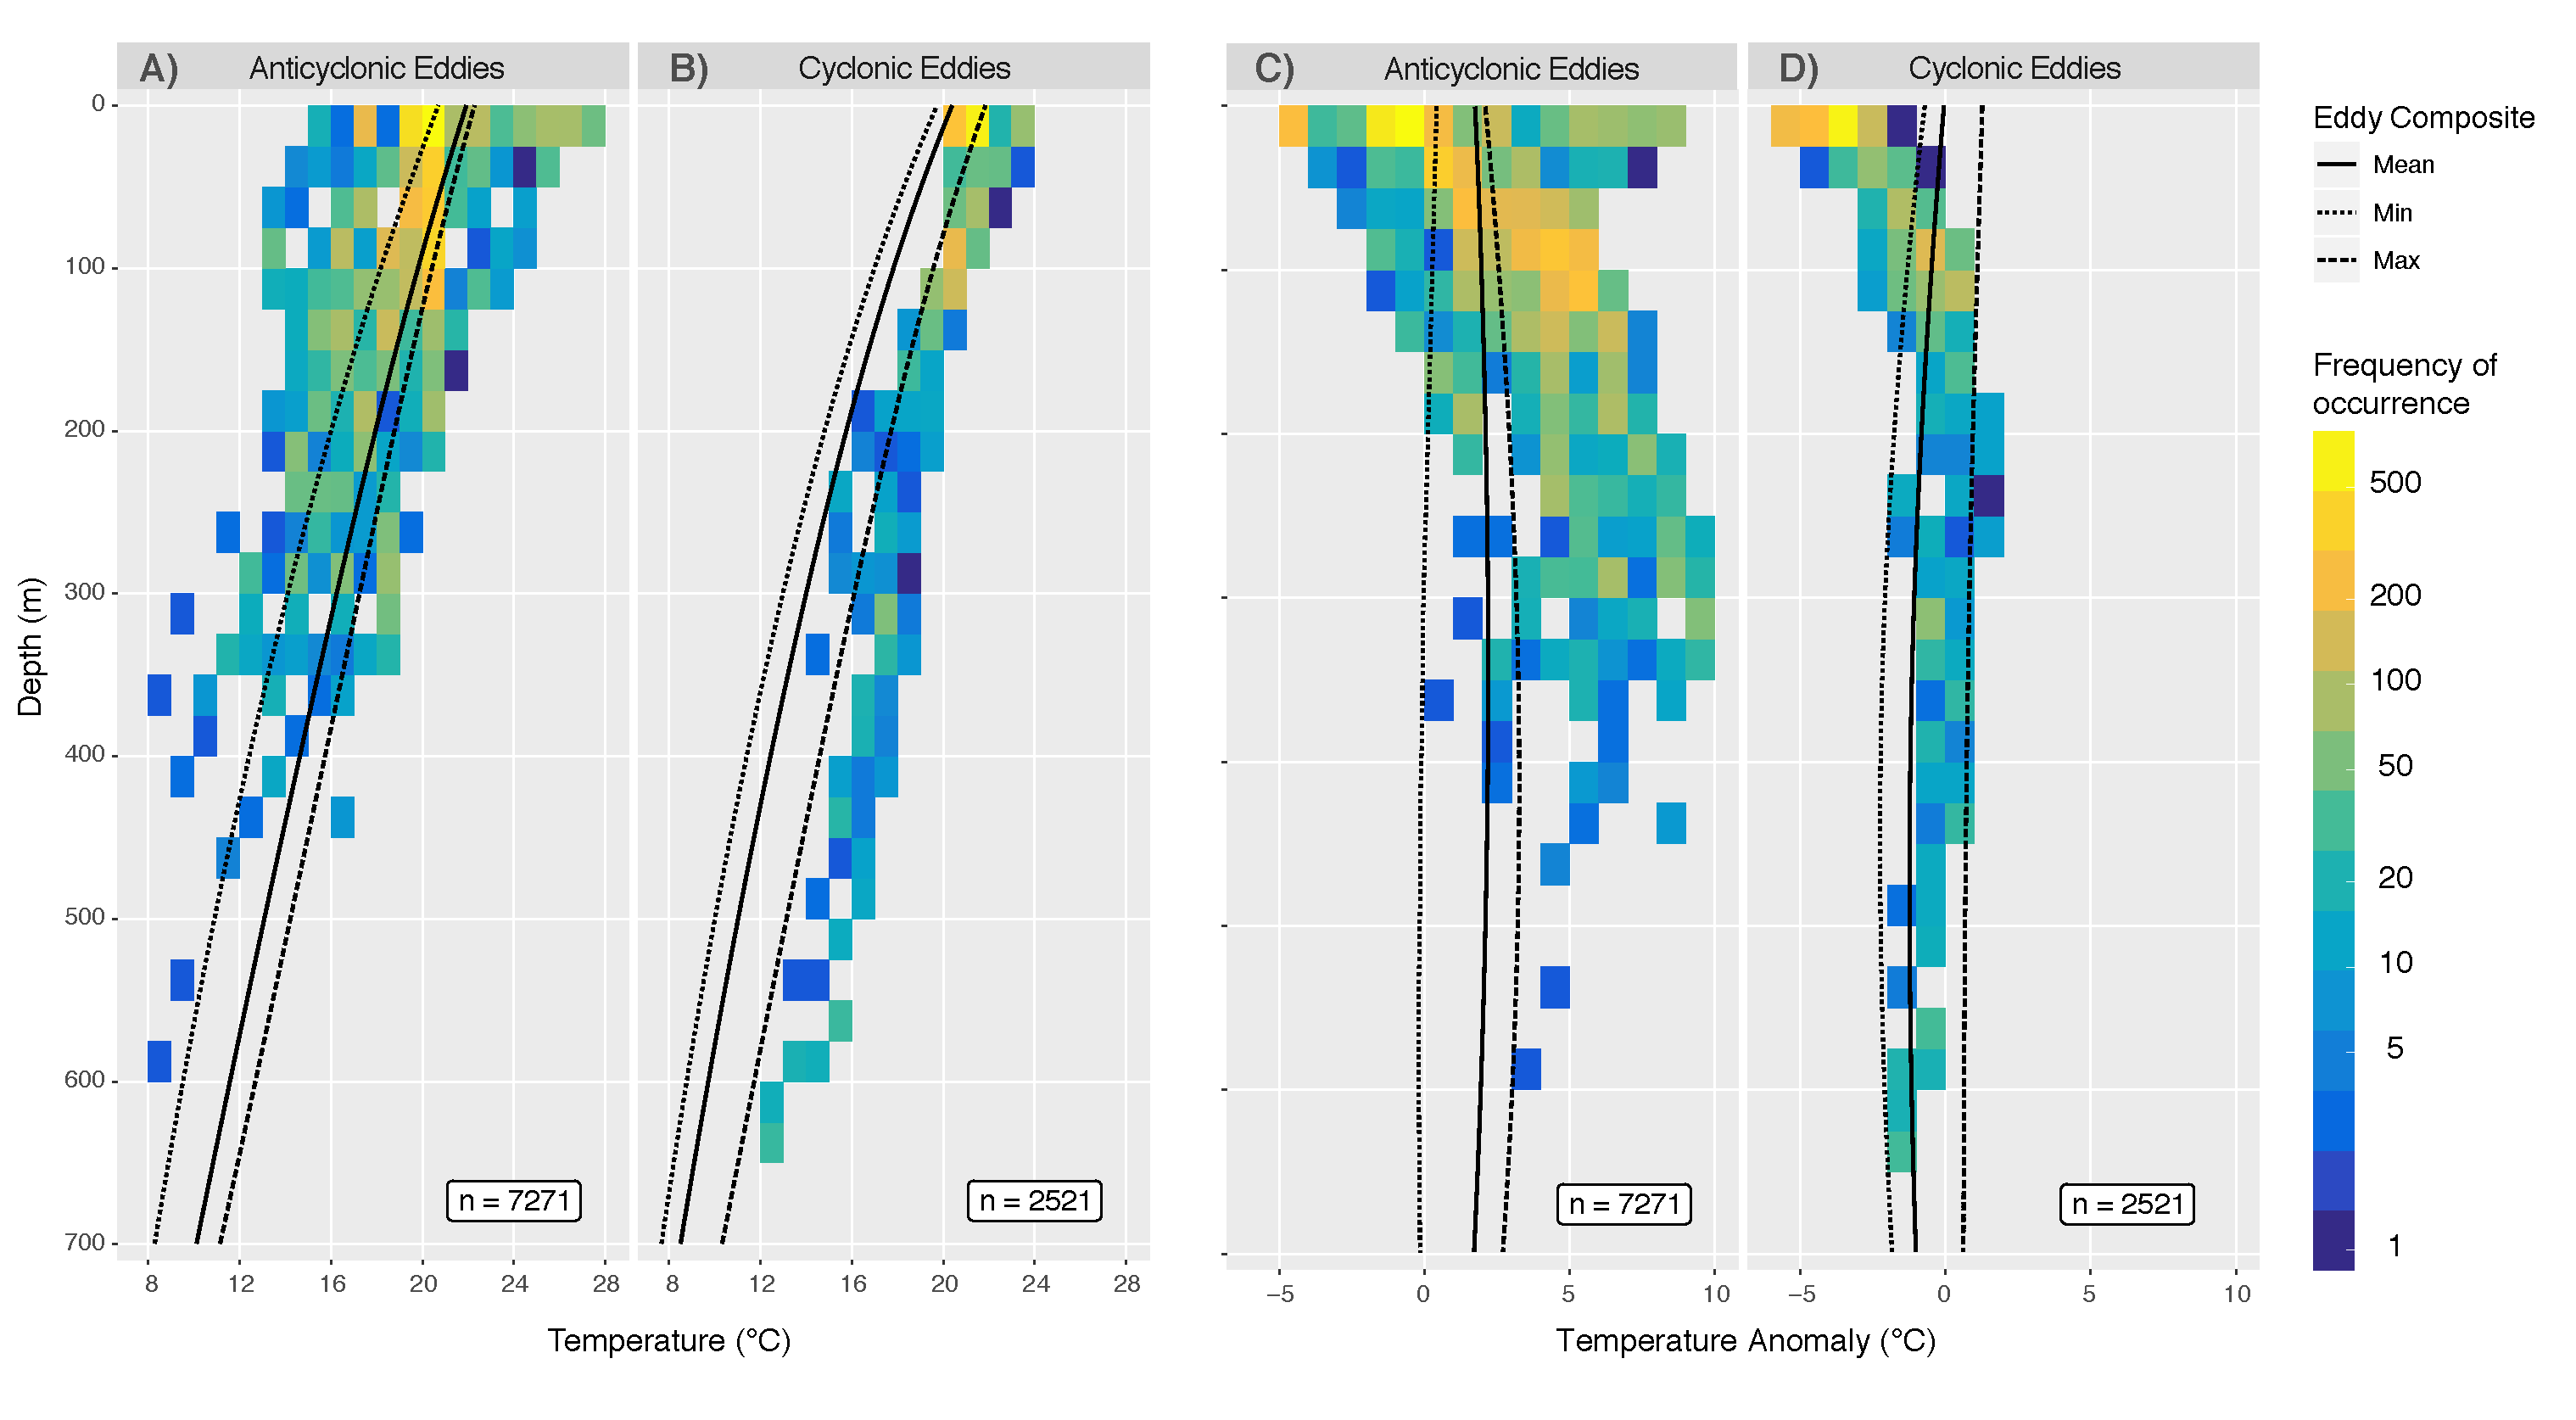
\includegraphics[width=\textwidth]{images/A5_Fig1.pdf}
\caption[Frequency of depth-temperature profile measurements recorded by PSAT-tagged blue sharks]{Frequency of depth-temperature profile measurements recorded by PSAT-tagged blue sharks summarized into 1$^\circ$ and 25 m bins. Color (log scale) denotes frequency of depth-temperature measurements within a given bin and eddy type for tag-measured temperature (A,B) and temperature anomaly of tag temperature as compared to World Ocean Atlas 2013 (C,D). Lines show mean and range of depth-temperature values from the HYCOM-derived eddy composites (see Figs. \ref{fig:c5f2}, \ref{fig:a5f2}). Tag-measured depth-temperature data is from inner-core ($r \leq L_s/2$) of eddies only.}
\label{fig:a5f1} %eddypdt
\end{figure}

\clearpage

%-------------------------

%\thispagestyle{empty}
\begin{figure}[htbp]
\centering
\includegraphics[width=.7\textwidth]{images/A5_Fig2.pdf}
\caption[Depth-temperature composite and anomaly for Gulf Stream eddies]{Depth-temperature composite for Gulf Stream anticyclones (A) and cyclones (B) derived from HYCOM-modeled temperature fields and anticyclone (D) and cyclone (E) composite temperature anomalies. Dashed vertical lines indicate eddy core and horizontal labeled lines indicate isotherms.}
\label{fig:a5f2} %vertanom
\end{figure}

\clearpage

%--------------------------
